\section*{Teoretická část}
Budeme studovat kmity dvou fyzických kyvadel vázaných slabou pružinou upevněnou ve vzdálenosti $l$ od uložení závěsů kyvadel (viz obrázek \ref{obr::aparatura}).
Po upevnění pružiny se rovnovážná poloha obou kyvadel vychýlí ze svislého směru o úhel $\alpha$ směrem k sobě.
Okamžitou výchylku $\varphi _1(t)$ resp. $\varphi _2 (t)$ uvažujeme od této nové rovnovážné polohy.

\begin{figure}[htbp]
\centering
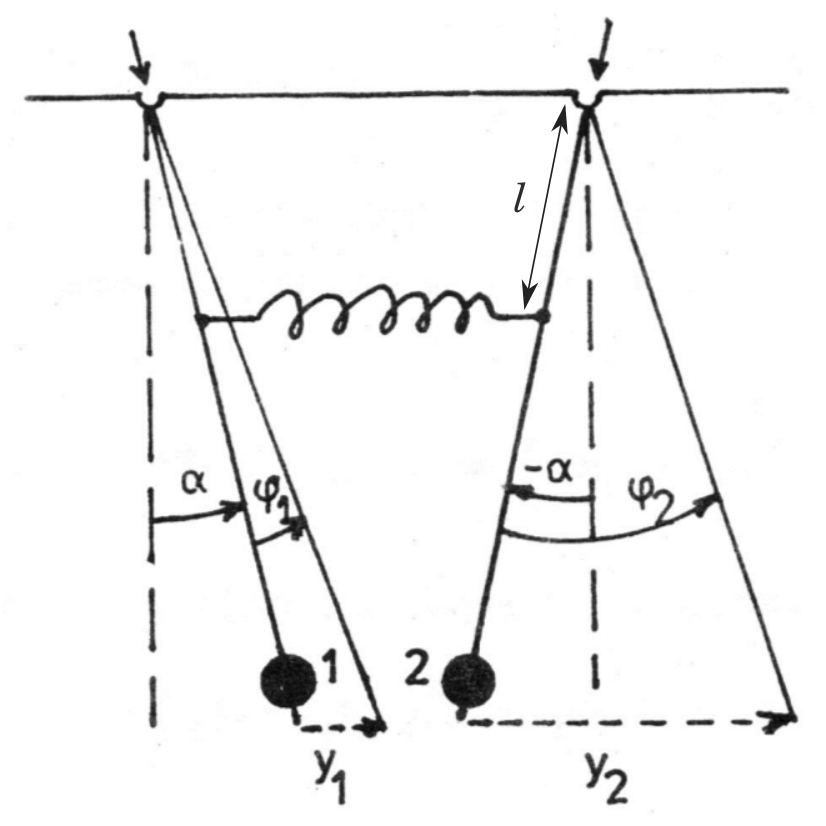
\includegraphics[width=\textwidth-9cm]{graficos/aparatura}
\caption{Nákres experimentu (přezato z \cite{ZFP})}
\label{obr::aparatura}
\end{figure}

Po vyřešení pohybových rovnic dostáváme pro malé výchylky \cite{ZFP}
\begin{align}
\label{eq::phiobecne}
\begin{split}
 \varphi _1(t) &= a_1 \cos (\omega _1 t) + b_1 \sin (\omega _1 t) + a_2 \cos (\omega_2 t) + b_2 \sin(\omega_2 t)
\\
 \varphi _2(t) &= a_1 \cos (\omega _1 t) + b_1 \sin (\omega _1 t) - a_2 \cos (\omega_2 t) - b_2 \sin(\omega_2 t) \,,
\end{split}
\end{align}
kde $a_1$, $b_1$, $a_2$ a $b_2$ jsou integrační konstanty, které určíme z~počátečních podmínek.
Úhlové frekvence $\omega _1$ a $\omega _2$ můžeme vypočítat podle vzorce \cite{ZFP}
\begin{align}
\label{eq::omegadirekcni}
\begin{split}
 \omega_1 &= \sqrt{\frac{D}{I}}
\\
 \omega_2 &= \sqrt{\frac{D+2D^{\ast}}{I}} \,,
\end{split}
\end{align}
kde $I$ je moment setrvačnosti kyvadla, $D$ je direkční moment kyvadla a $D^{\ast}$ je direkční moment pružiny. Žádnou z~těchto veličin však nebudeme měřit a úhlové rychlosti $\omega _1$ a $\omega _2$ změříme přímo při vhodně zvolených počátečních podmínkách.

Pro různé počáteční podmínky vychází:
\begin{enumerate}
\item Pro $\varphi _1 (0) = \varphi _2 (0) = A$, $\dot{\varphi_1}(0)=\dot{\varphi_2}(0)=0$ dostáváme
\begin{equation} \label{eq::philist1}
\varphi _1 = \varphi _2 = A \cos(\omega _1 t)\,.
\end{equation}
\item Pro $\varphi _1 (0) = - \varphi _2 (0) = A$, $\dot{\varphi_1}(0)=\dot{\varphi_2}(0)=0$ dostáváme
\begin{equation} \label{eq::philist2}
\varphi _1 = - \varphi _2 = A \cos(\omega _2 t) \,.
\end{equation}
\item Pro $\varphi _1 (0) = 0$, $\varphi _2 (0) = A$, $\dot{\varphi_1}(0)=\dot{\varphi_2}(0)=0$ dostáváme
\begin{align}
\label{eq::philist3}
\begin{split}
 \varphi_1 &= A \sin(\omega_4 t) \cdot \sin(\omega_3 t)
\\
 \varphi_2 &= A \cos(\omega_4 t) \cdot \cos(\omega_3 t) \,,
\end{split}
\end{align}
kde
\begin{align}
\label{eq::omega34}
\begin{split}
 \omega_3 &= \frac{1}{2}(\omega_2 + \omega_1)
\\
 \omega_4 &= \frac{1}{2}(\omega_2 - \omega_1) \,.
\end{split}
\end{align}

Pokud je vazba slabá, je $\omega _2$ jen o málo větší než $\omega_1$ a pohyb kyvadel můžeme považovat za harmonický s~úhlovou frekvencí $\omega_3$ a v čase proměnnou amplitudou $A \sin(\omega_4 t)$ ($A \cos(\omega_4 t)$ pro druhé kyvadlo). 

\end{enumerate}

Pro úhlové rychlosti $\omega_1$, $\omega_2$ a $\omega_3$ označíme odpovídající periody $T_1$, $T_2$ a $T_3$ resp.
Dále zavedeme dobu $T_S$ jako polovinu periody odpovídající $\omega_4$. Platí tedy vztahy
\begin{align}
\label{eq::periodyvztahy}
 T_1 \omega_1 &= 2\pi & T_2 \omega_2 &=2\pi \nonumber \\
 T_3 \omega_3 &= 2\pi & T_S \omega_4 &=\pi
\end{align}

Standardní odchylku úhlové rychlosti počítáme vždy jako $\sigma_\omega=\omega \cdot \sigma_T / T$.

S nahlédnutím do \eqref{eq::philist3} je $T_S$ zřejmě doba mezi dvěma časy, kdy je amplituda kyvadla nulová (viz~obrázek~\ref{obr::tretipripad}).

\begin{figure}[htbp]
\centering
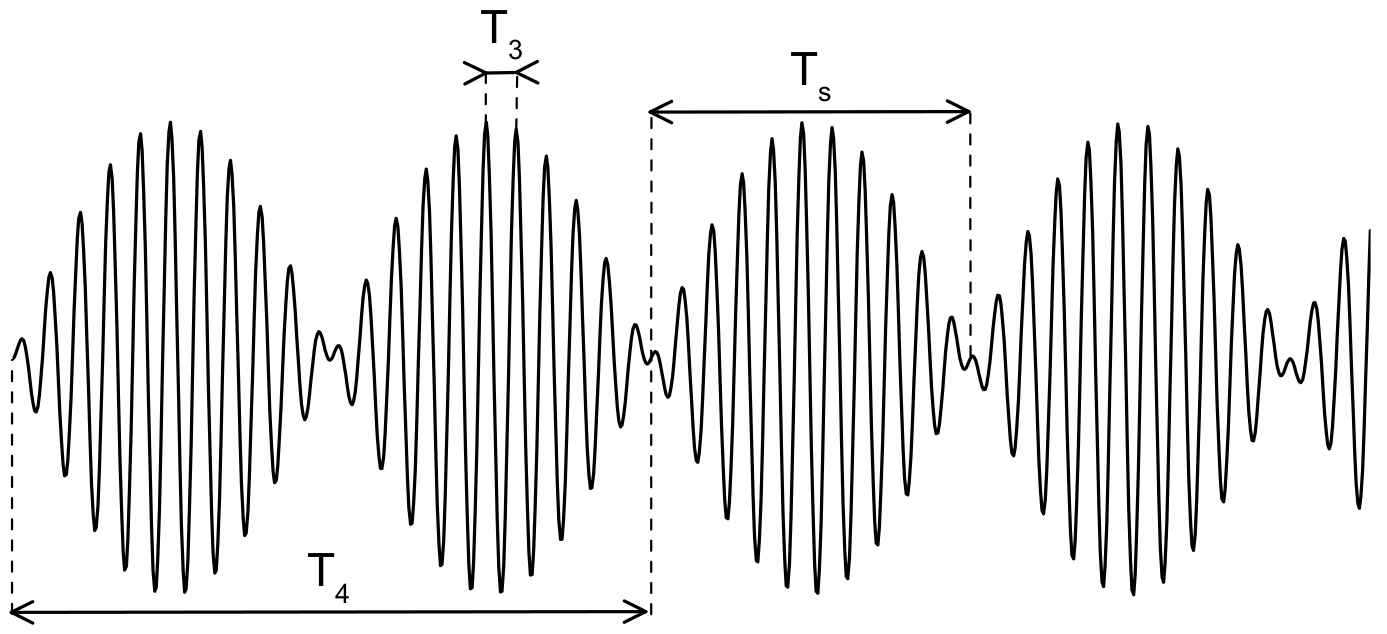
\includegraphics[width=\textwidth-2cm]{graficos/ts}
\caption{Časová závislost výchylky prvního kyvadla $\varphi_1$ při počátečních podmínkách $\varphi_1(0)=0$, $\varphi_2(0)=A$ a $\dot{\varphi_1}(0)=\dot{\varphi_2}(0)=0$, pokud zanedbáme tlumení. Závislost $\varphi_2$ je oproti $\varphi_1$ posunutá o čas $T_S/2$. Doba $T_4$ je perioda odpovídající úhlové rychlosti $\omega_4$ a platí $T_4=2T_S$. (převzato z \cite{ZFP})}
\label{obr::tretipripad}
\end{figure}

Stupeň vazby $\kappa$ je definován jako \cite{ZFP}
\begin{equation} \label{eq::kappadirekcni}
\kappa = \frac{D^{\ast}}{D+D^{\ast}} \,.
\end{equation} 

S využitím \eqref{eq::omegadirekcni} můžeme \eqref{eq::kappadirekcni} upravit na
\begin{equation}
\kappa = \frac{\omega_2^2-\omega_1^2}{\omega_2^2+\omega_1^2} \,.
\end{equation}

Standardní odchylku stupně vazby $\sigma_\kappa$ v závislosti na odchylkách $\sigma _{\omega_1}$ a $\sigma _{\omega_2}$ určíme jako
\begin{equation} \label{eq::odchylkakappa}
\sigma _\kappa = \sqrt{ \left( \frac{\partial \kappa}{\partial \omega_1} \right) ^2 \cdot \sigma_{\omega_1}^2    +   \left(  \frac{\partial \kappa}{\partial \omega_2}     \right)^2 \cdot \sigma_{\omega_2}^2    } = \frac{4 \omega_1^2 \omega_2^2}{ \left( \omega_1^2+\omega_2^2 \right) ^2} \sqrt{ \left( \frac{\sigma _{\omega_1}}{\omega_1}      \right)^2    +      \left( \frac{\sigma _{\omega_2}}{\omega_2}      \right)^2                   }
\end{equation}

